\documentclass[11pt,a4paper]{article}

% ---------------------------------------------------------------------------
% Prediction coverage in inherited-state branching models: an exact
% mean-closure counterexample, a repaired count threshold, and the effect of
% founder number.
%
% Author metadata: set the macros below before submission.  Author and
% affiliation are deliberately blank in this version.
% ---------------------------------------------------------------------------
\newcommand{\PaperAuthor}{}
\newcommand{\PaperAffiliation}{}
\newcommand{\PaperDate}{16 September 2026}
% Formal-status entries for the repair theorem (updated at build time).
\newcommand{\LeanRepairExact}{Compiled: \lean{PositiveRepair.lean}, \lean{actual_failure_ge_exact}: $\PP(N_T\ge3)\ge L$ with the exact rational $L$ of~\eqref{eq:L}, for the same founder mixture of chronological measures.}
\newcommand{\LeanRepair}{Compiled: \lean{PositiveRepair.lean}, root \lean{actual_repair_probability_ge}: $\PP(N_T\le3)\ge 467880212635/481696324816$ for the founder mixture of chronological measures, from a two-live-state killed chain for the sensitive founder (\lean{sensitiveSource}, \lean{finite_sensitive_exact}, value $\frac{300}{301}+\frac1{301}e^{-(30100/10001)\log2}$) and the resistant killed chain with payoff ``alive with at most three cells'' (\lean{finite_repair_exact}), both transported by \lean{stopped_clock_le_unrestricted}. Receipt $71.4$~s, axioms as above.}
\newcommand{\LeanMinimal}{Compiled: \lean{PositiveRepair.lean}, \lean{interval_two_undercovers}: the mixture probability of $\{N_T\le2\}$ is strictly below $19/20$, from the probability-measure complement of the tail event; together with the root above this is Corollary~\ref{cor:minimal} at the process level.}

\usepackage[T1]{fontenc}
\usepackage[utf8]{inputenc}
\usepackage{lmodern}
\usepackage{microtype}
\usepackage[a4paper,margin=1.05in]{geometry}
\usepackage{amsmath,amssymb,amsthm,mathtools}
\usepackage{booktabs}
\usepackage{array}
\usepackage{enumitem}
\usepackage{longtable}
\usepackage{graphicx}
\usepackage{xcolor}
\usepackage[obeyspaces,spaces]{url}
\usepackage[numbers,sort&compress]{natbib}
\usepackage[colorlinks=true,linkcolor=blue!55!black,citecolor=blue!55!black,urlcolor=blue!55!black]{hyperref}
\hypersetup{pdftitle={Prediction coverage in inherited-state branching models},
  pdfkeywords={branching processes, phenotypic switching, moment closure, prediction intervals, drug persistence, low-cell-count assays, Lean}}

\DeclareUrlCommand\lean{\urlstyle{tt}}
\setlist{itemsep=2pt,topsep=3pt}
\setlength{\emergencystretch}{1.5em}

\theoremstyle{plain}
\newtheorem{theorem}{Theorem}[section]
\newtheorem{proposition}[theorem]{Proposition}
\newtheorem{lemma}[theorem]{Lemma}
\newtheorem{corollary}[theorem]{Corollary}
\theoremstyle{definition}
\newtheorem{definition}[theorem]{Definition}
\theoremstyle{remark}
\newtheorem{remark}[theorem]{Remark}

\newcommand{\R}{\mathbb R}
\newcommand{\N}{\mathbb N}
\newcommand{\PP}{\mathbb P}
\newcommand{\EE}{\mathbb E}
\newcommand{\Var}{\operatorname{Var}}
\newcommand{\Cov}{\operatorname{Cov}}
\newcommand{\cL}{\mathcal L}
\newcommand{\dd}{\mathrm d}
\newcommand{\ind}{\mathbf 1}

\title{Prediction coverage in inherited-state branching models:\\ an exact mean-closure counterexample, a repaired count threshold,\\ and the effect of founder number}
\author{\PaperAuthor\\[2pt] {\small\itshape \PaperAffiliation}}
\date{\PaperDate}

\begin{document}
\maketitle

\begin{abstract}
Low-cell-count proliferation assays are often summarized by a scalar birth--death model whose per-cell rates are read off the expected phenotypic composition of the population. We show that such a mean-composition closure can reproduce the exact expected cell count, and even the exact expected birth and death fluxes, while assigning misleading probabilities to future counts. The witness is an explicit two-type branching process with positive switching in both directions, one founder of random type, and an observation horizon of one resistant doubling time. The scalar closure assigns probability at least $332/343>0.9679$ to the counts $\{0,1,2\}$, whereas the inherited-state process assigns them probability at most $1-L<0.95$ with $L=0.05044\ldots$ an explicit rational number. Both inequalities are proved analytically: the scalar tail is bounded through an explicit box for the mean and the accumulated-birth parameter, certified by one positive polynomial identity, and the actual tail is bounded from below by seven no-switch histories. Widening the region to $\{0,\dots,3\}$ restores coverage at least $H=0.9713\ldots$, and three is the smallest upper endpoint that reaches $95\%$ for this preparation. A variance comparison ($\Var Z_T\le 11/16<4/5<\Var N_T$) shows that the discrepancy does not disappear with many independent founders: the limiting actual coverage of the scalar central $95\%$ interval is below $0.9308$, and numerically about $0.849$. We give a general identity that expresses the variance defect of any mean-composition closure as an integrated covariance between population size and composition-weighted net growth, and closed low-count backward equations that compute corrected thresholds without solving the joint population law. Numerical checks reproduce the witness, scan the switching rates, exhibit the same mechanism with positive birth, death and day-scale switching in both states, and retain a source-linked preparation in which the closure performs well. The tail obstruction, the analytic box, the explicit scalar law and the repaired threshold are verified in Lean~4; the two process-identification bridges are proved conventionally and are identified as such. The witness is a synthetic persistent-state regime, not a fitted experiment.
\end{abstract}

\section{Introduction}\label{sec:intro}

\subsection{The question}
A low-founder proliferation assay produces a random cell count at a fixed time. A model can reproduce the average of that count over many replicate wells and still give the wrong probability for unusually small or unusually large outcomes. When cells inherit a phenotypic state at division, one founder's state influences the growth of its whole family, so a description that first averages the composition of the population and then computes fluctuations from that average may discard exactly the dependence that governs family sizes.

The specific closure we study is the following. A two-type process $(S_t,R_t)$ of sensitive and resistant cells has constant per-cell rates and exact type means $s(t)=\EE S_t$, $r(t)=\EE R_t$. The \emph{mean-composition closure} replaces it by a single-type birth--death process $Z_t$ whose per-cell birth and death rates at time $t$ are the population-average rates computed from $(s(t),r(t))$. By construction $\EE Z_t=\EE(S_t+R_t)$ for all $t$; the closure also matches the expected instantaneous birth and death fluxes. Closures of this kind are attractive in low-cell-count settings because they yield a one-dimensional master equation whose solution is available in closed form \citep{kendall1948,bailey1964}. \citet{browning2025} develop such an approximate count equation for a stochastic phenotype model and explicitly discuss the limitation introduced by phenotypic inheritance; \citet{iyer2025} show that inheritable states shape drug-persister correlations. The question addressed here is quantitative:

\begin{quote}
Can mean-composition closure invalidate a count-prediction region even when all rates and the initial preparation are known exactly and the expected count trajectory is matched exactly?
\end{quote}

The answer is yes, and the failure can be certified by hand. The witness is deliberately small. All of its probabilities are explicit rational or elementary expressions, the decisive inequalities are strict rational-arithmetic statements, and the argument never computes the full joint population law.

\subsection{Main results}
Section~\ref{sec:model} defines the process: sensitive cells die at rate $d=3/10$ per day, resistant cells divide at rate $b=1/10$ per day, sensitive cells switch to resistant at rate $\alpha=1/1000$ and resistant cells switch to sensitive at rate $\beta=1/100\,000$ per day; one founder is resistant with probability $5/24$. The horizon is $T=\log 2/(b+\beta)$, one resistant doubling time, and $c=b/(b+\beta)=10000/10001$.

\begin{enumerate}[label=(\roman*)]
\item \emph{Coverage failure with exact mean matching} (Theorem~\ref{thm:main}). $\EE Z_t=\EE N_t$ for all $t$, where $N_t=S_t+R_t$, yet
\[
\PP(Z_T\le2)\ \ge\ \tfrac{332}{343}>0.9679,\qquad
\PP(N_T\le2)\ \le\ 1-L<0.95,
\]
where $L=\tfrac5{48}\sum_{j=2}^6(\tfrac c2)^j=0.05044\ldots$ is an explicit rational number.
\item \emph{Instance-specific repair and minimality} (Theorem~\ref{thm:main}, Corollary~\ref{cor:minimal}). $\PP(N_T\le3)\ge H=0.97131\ldots$, an explicit rational number, and $3$ is the smallest $k$ for which $\{0,\dots,k\}$ has actual coverage at least $95\%$.
\item \emph{Persistence under many founders} (Proposition~\ref{prop:variance}, Theorem~\ref{thm:clt}). $\Var Z_T\le 11/16$ while $\Var N_T>4/5$. For $F$ independent founders the actual coverage of the scalar central $95\%$ interval converges to $2\Phi(z_{.975}\sqrt{v_Z/v_N})-1<2\Phi(z_{.975}\sqrt{55/64})-1<0.9308$.
\item \emph{What the closure discards} (Proposition~\ref{prop:defect}). For any finite-type process with constant per-cell rates and count-preserving switching, the variance defect of the mean-composition closure satisfies
\[
v_N(t)-v_Z(t)=2m(t)^2\int_0^t\frac{\Cov\bigl(N_u,\;G_u-\bar g(u)N_u\bigr)}{m(u)^2}\,\dd u ,
\]
where $G$ is the population net-growth propensity and $\bar g=\EE G/\EE N$. Inheritance therefore inflates variance exactly when population size covaries with composition-weighted excess growth; when all types have the same net growth rate the defect vanishes identically.
\item \emph{Computable corrections} (Proposition~\ref{prop:lowcount}). The probabilities $\PP(N_T=n)$ for $n\le k$ satisfy a closed system of $2(k+1)$ ordinary differential equations obtained from the backward generating-function equations. Corrected thresholds for other preparations, and for $F$ independent or binomially plated founders, follow without solving a two-dimensional master equation. A mean-only Markov bound would certify endpoint $10$ for the witness; the type-aware calculation certifies $3$.
\end{enumerate}
Section~\ref{sec:numerics} reproduces the witness numerically, tabulates independent-founder coverage, scans both switching rates over five decades, exhibits the mechanism with strictly positive birth, death and switching rates in both states and switching times of ten days, and reports a source-linked preparation from \citet{browning2025} in which the closure covers correctly. Section~\ref{sec:discussion} states what the result does and does not show.

\subsection{Relation to existing work}
The scalar terminal law used here is the linear-fractional law of the time-dependent birth--death process \citep{kendall1948,bailey1964}; nothing about it is new. Two-type Markov branching processes and their moment equations are classical \citep{harris1963,athreyaney1972,haccou2005}, and their use for drug resistance in cancer \citep{iwasa2006,bozic2013,durrett2015} and for phenotypic switching in bacteria \citep{balaban2004,kussell2005} is well established. That inherited traits generate correlated family sizes and excess variance in counts has been understood since \citet{luria1943}. Reversible drug-tolerant states in cancer cell subpopulations \citep{sharma2010,shaffer2017} motivate the two-type structure, and \citet{iyer2025} model inherited states and persister correlations directly. On the approximation side, moment-closure methods and their accuracy have been reviewed extensively \citep{singh2011,grima2012,schnoerr2017}, and identifiability from low-cell-count experiments is the subject of \citet{browning2020,browning2025}. Calibration of prediction intervals as a criterion in its own right is discussed by \citet{gneiting2007}.

Against this background the contribution of the present paper is not the existence of inherited-state correlations. It is (a) an explicit, fully certified example in which a mean-composition closure that matches the exact mean and the exact expected fluxes nevertheless fails a stated prediction-coverage requirement, with a small-event proof that avoids the joint population law; (b) the instance-specific corrected threshold and the proof that it is minimal in its family; (c) the founder-number limit, which shows that the failure is a variance-ratio error preserved by the central limit theorem rather than a small-count artefact; (d) the variance-defect identity, which locates the failure in one covariance and gives a sign condition; and (e) the low-count backward equations as a practical route to corrected thresholds in the same model class.

\subsection{Scope, methods and verification}
All probabilities concern repeated realizations of a process with known, fixed rate parameters. A prediction region covers a future cell count; it is neither a confidence interval for an estimated parameter nor a posterior credible interval. The population is well mixed and non-interacting, with exponential event times, no immigration, no density dependence, no observation error and no shared random environment. The witness is a synthetic persistent-state regime and is not a calibration of any experiment.

Every inequality in Theorems~\ref{thm:main} and \ref{thm:clt} and Propositions~\ref{prop:variance}, \ref{prop:defect} and \ref{prop:lowcount} is proved in the text. The actual-process tail obstruction, the nonexplosive process law it is stated for, the analytic bounds on the first-moment system, the explicit scalar law with its normalization and its $332/343$ coverage, and the process-level repaired threshold are additionally verified in Lean~4 with Mathlib \citep{demoura2021,mathlib2020}; Appendix~\ref{app:lean} lists the declarations and what they do and do not cover. Two bridges remain conventional: that the unrestricted process means coincide with the ODE solution, and that the time-inhomogeneous scalar jump process has the explicit terminal law. Both are standard and both are proved in Section~\ref{sec:proof}; we describe the development as a conventional proof with machine-checked components. The script \path{check_paper.py} distributed with the sources replays every constant printed below in exact rational arithmetic and regenerates the figures and floating-point diagnostics.

\section{Model, closure and statistical target}\label{sec:model}

\subsection{The inherited-state process}
Let $X_t=(S_t,R_t)\in\N_0^2$ be a continuous-time Markov chain with the transitions of Table~\ref{tab:rates}. A division adds one cell of the parent's current type, equivalently replaces the parent by two cells of that type; a switch changes the type of one cell and preserves the total count $N_t=S_t+R_t$. Cells interact only through genealogy: given the current state, every cell acts independently. There is exactly one founder, whose type is drawn once,
\begin{equation}\label{eq:initial}
\PP\bigl(X_0=(1,0)\bigr)=\tfrac{19}{24},\qquad \PP\bigl(X_0=(0,1)\bigr)=\tfrac5{24}.
\end{equation}
The founder's type is not redrawn at later events; the descendants inherit the current type of their parent and switch independently thereafter. This is the mechanism under study.

\begin{table}[ht]
\centering
\caption{Transitions of the witness. All per-cell rates are in day$^{-1}$; sensitive division and resistant death have rate zero in the exact witness (Section~\ref{sec:numerics} relaxes this numerically).}
\label{tab:rates}
\begin{tabular}{llll}
\toprule
Event & Change in $(S,R)$ & Total intensity & Parameter\\
\midrule
Sensitive death & $(-1,0)$ & $dS$ & $d=3/10$\\
Resistant division & $(0,+1)$ & $bR$ & $b=1/10$\\
Sensitive $\to$ resistant & $(-1,+1)$ & $\alpha S$ & $\alpha=1/1000$\\
Resistant $\to$ sensitive & $(+1,-1)$ & $\beta R$ & $\beta=1/100\,000$\\
\bottomrule
\end{tabular}
\end{table}

The observation horizon and a recurring constant are
\begin{equation}\label{eq:horizon}
T=\frac{\log2}{b+\beta}=6.9307787\ldots\ \text{days},\qquad c=\frac b{b+\beta}=\frac{10000}{10001}.
\end{equation}
Thus $T$ is one doubling time of an isolated resistant lineage, and $c$ is the probability that the next event of a resistant cell is a division rather than a switch.

\subsection{Mean-composition closure}
Write $s(t)=\EE S_t$, $r(t)=\EE R_t$ and $m(t)=s(t)+r(t)$. Lemma~\ref{lem:moments} shows that these are finite, that $m(t)>0$, and that they solve the linear system~\eqref{eq:means}. The scalar closure is the time-inhomogeneous birth--death process $Z_t$ on $\N_0$ with $Z_0=1$, birth intensity $\lambda(t)Z_t$ and death intensity $\delta(t)Z_t$, where
\begin{equation}\label{eq:rates}
\lambda(t)=\frac{b\,r(t)}{m(t)},\qquad \delta(t)=\frac{d\,s(t)}{m(t)} .
\end{equation}
These are the per-cell birth and death rates of a population whose composition is replaced by its expected composition. They are deterministic functions of time computed from the exact means, not from a fitted or estimated trajectory, and they differ in general from rates conditional on the realized count. Once mean matching is established (Lemma~\ref{lem:moments}),
\[
\lambda(t)\,\EE Z_t=b\,\EE R_t,\qquad \delta(t)\,\EE Z_t=d\,\EE S_t ,
\]
so the closure also reproduces the expected birth and death fluxes at every time. Whatever it gets wrong is therefore not the average flux; it is the distribution and dependence structure that averaging removes.

\subsection{Prediction regions}
Two constructions are relevant. A one-sided integer region $\{0,\dots,k\}$ is acceptable at level $95\%$ when its probability under the governing law is at least $0.95$; Theorem~\ref{thm:main} treats the regions with $k=2$ and $k=3$ analytically. A \emph{central} scalar quantile interval has endpoints at the $2.5\%$ and $97.5\%$ integer quantiles of the scalar law; it is the construction a user of the closure would report. For the witness the scalar central $95\%$ interval is $[0,2]$ numerically (Section~\ref{sec:numerics}). The analytic bound $\PP(Z_T\ge3)\le 11/343$ alone does not certify that identification, because $11/343>0.025$; we keep the analytic statement about $\{0,1,2\}$ separate from the numerical quantile calculation.

\subsection{Physical scale of the witness}
The sensitive death time is $1/d\approx3.3$ days and the resistant doubling time is $T\approx6.93$ days. The isolated switching clocks have means $1/\alpha=1000$ days and $1/\beta=100\,000$ days, so $\alpha T\approx0.0069$ and $\beta T\approx0.0000693$: over the horizon a switch is rare, and the founder's state is effectively inherited by its whole family. This is a persistent-state stress test, and it must not be read as a measured reversible switching rate. Rescaling every rate and the horizon by a common factor changes units but not the ratios that matter. Sections~\ref{sec:grid}--\ref{sec:positive} examine numerically what happens when the switching clocks are shortened to days and when every event class has a positive rate.

\section{Main theorem}\label{sec:main}

\begin{theorem}[Coverage failure and its repair]\label{thm:main}
For the processes of Section~\ref{sec:model}, $\EE Z_t=\EE N_t$ for all $t\ge0$. At the horizon $T$ of~\eqref{eq:horizon},
\begin{align}
\PP(Z_T\le2)&\ \ge\ \frac{332}{343}=0.96793\ldots,\label{eq:scalarclaim}\\
\PP(N_T\le2)&\ \le\ 1-L<0.95,\label{eq:trueclaim}\\
\PP(N_T\le3)&\ \ge\ H>0.9713,\label{eq:repairclaim}
\end{align}
where
\begin{align}
L&=\frac5{48}\sum_{j=2}^{6}\Bigl(\frac c2\Bigr)^{j}
=\frac{151415045117539070312500}{3001800450060004500180003}=0.050441409293\ldots,\label{eq:L}\\
H&=\frac{19}{24}\cdot\frac{300}{301}+\frac5{48}\Bigl(1+\frac c2+\Bigl(\frac c2\Bigr)^2\Bigr)
=\frac{467880212635}{481696324816}=0.971317796152\ldots\label{eq:H}
\end{align}
\end{theorem}

\begin{corollary}[Minimal upper endpoint]\label{cor:minimal}
Among the regions $\{0,\dots,k\}$, $k\in\N_0$, the smallest $k$ whose coverage under the inherited-state process is at least $95\%$ is $k=3$. The scalar closure, by contrast, already attributes more than $96.79\%$ to $k=2$.
\end{corollary}
\begin{proof}
Coverage is nondecreasing in $k$; \eqref{eq:trueclaim} rules out every $k\le2$ and \eqref{eq:repairclaim} admits $k=3$.
\end{proof}

\begin{remark}[What the certified numbers mean]
The certified gap between the two models on $\{0,1,2\}$ is at least $L-11/343=0.01837\ldots$, about $1.84$ percentage points. The certified amount by which the actual coverage misses $95\%$ is smaller, at least $L-1/20=0.00044\ldots$. Numerically the actual coverage of $\{0,1,2\}$ is $0.94760$, so the true shortfall is about $0.24$ percentage points and the true gap about $2.9$ points. Remark~\ref{rem:geometric} sharpens the certified shortfall to $0.00207$ with a geometric series. The corollary concerns the family $\{0,\dots,k\}$ only; it does not assert that $\{0,\dots,3\}$ is the shortest prediction set, an equal-tailed interval, or a universal add-one rule.
\end{remark}

\section{Proof of Theorem~\ref{thm:main}}\label{sec:proof}

\subsection{Nonexplosion and exact first moments}\label{sec:moments}

\begin{lemma}[Yule domination and mean equations]\label{lem:moments}
The process $X$ is nonexplosive. On a common probability space there is a Yule process $Y$ with per-cell rate $b$ and $Y_0=1$ such that $\sup_{u\le t}N_u\le Y_t$ almost surely; in particular
\begin{equation}\label{eq:yule}
\EE\sup_{u\le t}N_u\le\EE Y_t=e^{bt},\qquad \EE\sup_{u\le t}N_u^2\le\EE Y_t^2=2e^{2bt}-e^{bt}.
\end{equation}
The means $s,r$ are finite, continuously differentiable, and are the unique solution of
\begin{equation}\label{eq:means}
\begin{pmatrix}s'\\ r'\end{pmatrix}
=\begin{pmatrix}-(d+\alpha)&\beta\\ \alpha&b-\beta\end{pmatrix}\begin{pmatrix}s\\ r\end{pmatrix},
\qquad \begin{pmatrix}s(0)\\ r(0)\end{pmatrix}=\begin{pmatrix}19/24\\ 5/24\end{pmatrix},
\end{equation}
that is, with the witness rates, $s'=-\frac{301}{1000}s+\frac1{100000}r$ and $r'=\frac1{1000}s+\frac{9999}{100000}r$.
Moreover $m(t)>0$ for every $t\ge0$. The scalar process $Z$ is well defined and nonexplosive, is dominated by the same kind of Yule process, and $\EE Z_t=m(t)$ for all $t$.
\end{lemma}

\begin{proof}
\emph{Embedding.} Construct the population inside a Yule tree of per-cell rate $b$ started from one cell, as follows. Every biological cell alive at time $t$ is attached to a distinct Yule cell. Each Yule cell carries an exponential($b$) division clock; when the clock of a Yule cell attached to a resistant biological cell rings, both the Yule cell and the biological cell divide, and the two new biological cells are attached to the two new Yule cells. When the clock of a Yule cell attached to a sensitive biological cell rings, or of a Yule cell with no attachment, only the Yule cell divides; its children are unattached. Each biological cell additionally carries independent exponential clocks for death (rate $d$ if sensitive, $0$ if resistant) and for switching (rate $\alpha$ if sensitive, $\beta$ if resistant); death removes the biological cell and leaves its Yule cell unattached, and switching relabels the cell. By the memoryless property this construction realizes the chain of Table~\ref{tab:rates}, the attached cells are always a subset of the Yule cells, and $N_u\le Y_u\le Y_t$ for $u\le t$. The Yule process is nonexplosive \citep[Chapter~2]{norris1997}, and on any bounded interval the finitely many Yule cells bound the total intensity of all death and switching clocks, so the biological process has finitely many events on bounded intervals as well. The moments in~\eqref{eq:yule} are the classical Yule moments, obtained by applying the pure-birth generator to $n$ and $n^2$ or from the geometric law of $Y_t$ \citep{yule1925,kendall1948}.

\emph{Stopped generator identity.} Let $\tau_K=\inf\{t:N_t>K\}$. Every transition changes $N$ by at most one, so the stopped process $X_{t\wedge\tau_K}$ takes values in the finite set $\{N\le K+1\}$ and Dynkin's formula for it is a finite-state identity requiring no interchange of limits \citep[Chapter~4]{ethierkurtz1986}:
\[
\EE S_{t\wedge\tau_K}=\tfrac{19}{24}+\EE\int_0^{t\wedge\tau_K}\bigl(-(d+\alpha)S_u+\beta R_u\bigr)\,\dd u,
\qquad
\EE R_{t\wedge\tau_K}=\tfrac5{24}+\EE\int_0^{t\wedge\tau_K}\bigl(\alpha S_u+(b-\beta)R_u\bigr)\,\dd u .
\]
As $K\to\infty$, $\tau_K\to\infty$ by nonexplosion; the stopped coordinates are bounded by $Y_t$ and the integrands by $(d+\alpha+\beta+b)\,Y_t$, both integrable by~\eqref{eq:yule}. Dominated convergence on the endpoint and on the time integral removes the stopping and gives the integral form of~\eqref{eq:means}. The integrands are bounded by an integrable function uniformly in $u\le t$, so $s$ and $r$ are continuous, hence the integral equations make them continuously differentiable, and the linear system~\eqref{eq:means} has a unique solution. Positivity of $m$: with probability at least $\frac5{24}e^{-(b+\beta)t}>0$ a resistant founder has no event before $t$, so $\PP(N_t\ge1)>0$ and $m(t)>0$.

\emph{Scalar process.} By Lemma~\ref{lem:box} below, or simply by nonnegativity of $s,r$ and $m>0$, the rates~\eqref{eq:rates} are continuous with $0\le\lambda\le b$ and $0\le\delta\le d$. The same embedding (attach each scalar cell to a Yule cell, accept a Yule division at time $u$ with probability $\lambda(u)/b$ independently, and run independent death clocks of rate $\delta(u)$) produces a nonexplosive process with the prescribed intensities, dominated by $Y$. The stopped identity gives $\EE Z_{t\wedge\tau_K}=1+\EE\int_0^{t\wedge\tau_K}(\lambda(u)-\delta(u))Z_u\,\dd u$, and dominated convergence yields $(\EE Z)'=(\lambda-\delta)\EE Z$ with $\EE Z_0=1$. From~\eqref{eq:means}, $m'=br-ds=(\lambda-\delta)m$ with $m(0)=1$, so $\EE Z_t=m(t)$ by uniqueness for this scalar linear equation.
\end{proof}

\subsection{The scalar terminal law}\label{sec:scalarlaw}
Define the accumulated-birth parameter
\begin{equation}\label{eq:A}
A(t)=m(t)\int_0^t\frac{\lambda(u)}{m(u)}\,\dd u .
\end{equation}
Since $m'=(\lambda-\delta)m$, $A'=\lambda+(\lambda-\delta)A$, and differentiating $1/m$ gives the normalization identity
\begin{equation}\label{eq:positive}
1+A(t)-m(t)=m(t)\int_0^t\frac{\delta(u)}{m(u)}\,\dd u\ \ge0 .
\end{equation}

\begin{lemma}[Kendall's law for the closure]\label{lem:scalar}
Write $m=m(T)$ and $A=A(T)$. For $0\le z\le1$,
\begin{equation}\label{eq:pgf}
\EE z^{Z_T}=1-\frac{m(1-z)}{1+A(1-z)} ,
\end{equation}
so that
\begin{equation}\label{eq:weights}
\PP(Z_T=0)=w_0=1-\frac m{1+A},\qquad \PP(Z_T=n)=w_n=\frac m{(1+A)^2}\Bigl(\frac A{1+A}\Bigr)^{n-1}\quad(n\ge1),
\end{equation}
and in particular
\begin{equation}\label{eq:tailvar}
\PP(Z_T\ge3)=\frac{mA^2}{(1+A)^3},\qquad \Var Z_T=m(1+2A)-m^2 .
\end{equation}
\end{lemma}

\begin{proof}
The law~\eqref{eq:pgf} is the classical linear-fractional law of the time-dependent birth--death process \citep{kendall1948}. We include a proof that identifies it with the process constructed in Lemma~\ref{lem:moments} without assuming uniqueness of an infinite forward system. Fix $z\in(0,1)$ and, for $0\le u\le T$, set
\[
M_u=\frac{m(T)}{m(u)},\qquad B_u=m(T)\int_u^T\frac{\lambda(v)}{m(v)}\,\dd v,\qquad h(u)=1-\frac{M_u(1-z)}{1+B_u(1-z)} .
\]
Integrating $(1/m)'=-(\lambda-\delta)/m$ over $[u,T]$ and multiplying by $m(T)$ gives $1+B_u-M_u=m(T)\int_u^T\delta/m\,\dd v\ge0$, so $M_u(1-z)\le(1+B_u)(1-z)\le1+B_u(1-z)$ and $0\le h(u)\le1$. Direct differentiation with $M_u'=-(\lambda-\delta)M_u$ and $B_u'=-\lambda M_u$ gives
\begin{equation}\label{eq:riccati}
h'(u)=\bigl(\lambda(u)h(u)-\delta(u)\bigr)\bigl(1-h(u)\bigr),\qquad h(T)=z .
\end{equation}
Let $f(u,n)=h(u)^n$ with $f(u,0)=1$. The scalar generator at time $u$ acts by $\cL_uf(u,n)=\lambda(u)n\,(h^{n+1}-h^n)+\delta(u)n\,(h^{n-1}-h^n)=n h^{n-1}(1-h)(\delta-\lambda h)$, so by~\eqref{eq:riccati} $(\partial_u+\cL_u)f=0$. Stop $Z$ at $\tau_K=\inf\{u:Z_u>K\}$; the stopped process lives on $\{0,\dots,K+1\}$, the rates are continuous, and $f$ is $C^1$ in $u$, so the finite-state time-inhomogeneous Dynkin formula gives $\EE f(T\wedge\tau_K,Z_{T\wedge\tau_K})=f(0,1)=h(0)$. Since $0\le f\le1$ and $\tau_K\to\infty$, bounded convergence gives $\EE z^{Z_T}=h(0)$. At $u=0$, $M_0=m(T)$ and $B_0=A(T)$, which is~\eqref{eq:pgf} for $z\in(0,1)$; the endpoints $z=0,1$ follow by monotone convergence, avoiding any convention at $0^0$. Expanding~\eqref{eq:pgf} in powers of $z$ gives~\eqref{eq:weights}; the geometric series sums the weights to one, and~\eqref{eq:positive} makes $w_0\ge0$. Finally $1-w_0-w_1-w_2=mA^2/(1+A)^3$ and $\Var Z_T=G''(1)+G'(1)-G'(1)^2=2mA+m-m^2$ with $G$ the right-hand side of~\eqref{eq:pgf}.
\end{proof}

\subsection{An explicit analytic box}\label{sec:box}

\begin{lemma}[Box for the mean and the birth parameter]\label{lem:box}
$0<m(T)\le 11/20$ and $0\le A(T)\le 2/5$.
\end{lemma}

\begin{proof}
Let $m_0(t)=\frac{19}{24}e^{-3t/10}+\frac5{24}e^{t/10}$ be the total mean of the same system with $\alpha=\beta=0$. Integrating factors in~\eqref{eq:means} give, for $0\le t\le7$,
\begin{align}
m(t)&\le e^{t/10}, & r(t)&\le\frac{26}{25}\cdot\frac5{24}\,e^{t/10},\label{eq:bounds1}\\
s(t)&\le\frac{19}{24}e^{-3t/10}+\frac1{40000}e^{t/10}, & m(t)&\ge\frac{993}{1000}\,m_0(t).\label{eq:bounds2}
\end{align}
Indeed $m'=br-ds\le bm$ gives the first bound. Then $r'=\alpha s+(b-\beta)r\le\alpha e^{bt}+br$, so $(e^{-bt}r)'\le\alpha$ and $e^{-bt}r\le\frac5{24}+7\alpha=\frac5{24}+\frac7{1000}<\frac{26}{25}\cdot\frac5{24}$. Next $s'\le-ds+\beta r\le-ds+\beta e^{bt}$, so $(e^{dt}s)'\le\beta e^{(b+d)t}$ and $s\le\frac{19}{24}e^{-dt}+\frac{\beta}{b+d}e^{bt}$ with $\beta/(b+d)=1/40000$. For the lower bound keep only the diagonal terms, $s\ge\frac{19}{24}e^{-(d+\alpha)t}$ and $r\ge\frac5{24}e^{(b-\beta)t}$, and use $e^{-\beta t}\ge e^{-\alpha t}\ge1-\alpha t\ge993/1000$.

\emph{Mean.} Since $T<7$ we have $e^{T/10}=2^{c}\le2$, and $e^{-3T/10}=2^{-3c}=\frac18e^{3\beta T}\le\frac18\cdot\frac{1001}{1000}$ because $3\beta T<21/100000$ and $e^x\le(1-x)^{-1}<1001/1000$ there. Adding the bounds on $s(T)$ and $r(T)$,
\[
m(T)\le\frac{19}{24}\cdot\frac{1001}{8000}+\frac1{20000}+\frac{26}{25}\cdot\frac5{24}\cdot2=0.53244\ldots<\frac{11}{20}.
\]

\emph{Birth parameter.} By~\eqref{eq:A} and~\eqref{eq:rates}, $A(T)=m(T)\int_0^T b\,r(u)/m(u)^2\,\dd u$. Substitute $x=e^{u/10}-1$, so $\dd u=10\,\dd x/(1+x)$ and $x\le e^{T/10}-1\le1$, and write $D(x)=5(1+x)^4+19$, so that $m_0(10\log(1+x))=D(x)/(24(1+x)^3)$. Inserting~\eqref{eq:bounds1}--\eqref{eq:bounds2} and $\frac5{24}\cdot24^2=120$,
\begin{equation}\label{eq:Abound}
A(T)=m(T)\int_0^{e^{T/10}-1}\frac{r(10\log(1+x))}{(1+x)\,m(10\log(1+x))^2}\,\dd x
\le\frac{11}{20}\cdot\frac{26/25}{(993/1000)^2}\int_0^1\frac{120(1+x)^6}{D(x)^2}\,\dd x .
\end{equation}
Let $I=\int_0^1\bigl[120(1+x)^6+1368(1+x)^2\bigr]/D(x)^2\,\dd x$. With $\mu_0(x)=D(x)/(24(1+x)^3)$ one checks $(1/\mu_0)'=[1368(1+x)^2-120(1+x)^6]/D(x)^2$ and $1/\mu_0(1)-1/\mu_0(0)=31/33$, hence
\[
\int_0^1\frac{120(1+x)^6}{D(x)^2}\,\dd x=\frac12\Bigl(I-\frac{31}{33}\Bigr)\le\frac{173}{264},
\]
where the inequality uses $I\le 9/4$, proved in Appendix~\ref{app:certificate} by one positive polynomial identity. Substituting in~\eqref{eq:Abound},
\[
A(T)\le\frac{11}{20}\cdot\frac{26}{25}\cdot\Bigl(\frac{1000}{993}\Bigr)^2\cdot\frac{173}{264}=\frac{1124500}{2958147}=0.38013\ldots<\frac25 . \qedhere
\]
\end{proof}

\begin{remark}
The box is deliberately coarse. The numerical values are $m(T)=0.51862$ and $A(T)=0.32163$ (Table~\ref{tab:witness}); the exact value of $I$ is $2.1788$, against the certified $132541/60000=2.2090$. A sharper box would sharpen~\eqref{eq:scalarclaim} but would not change the decision, and the polynomial certificate is the only auxiliary inequality the proof needs.
\end{remark}

\subsection{The scalar tail}
The function $a\mapsto a^2/(1+a)^3$ has derivative $a(2-a)/(1+a)^4\ge0$ on $[0,2]$, so it is nondecreasing on $[0,2/5]$. By~\eqref{eq:tailvar} and Lemma~\ref{lem:box},
\begin{equation}\label{eq:scalartail}
\PP(Z_T\ge3)=\frac{m(T)A(T)^2}{(1+A(T))^3}\le\frac{(11/20)(2/5)^2}{(7/5)^3}=\frac{11}{343},
\end{equation}
which is~\eqref{eq:scalarclaim}.

\subsection{The actual tail from seven histories}\label{sec:actualtail}
Start from one resistant cell and kill the process at its first switching event. Before killing, the population is a pure-birth process in which each of the $n$ cells divides at rate $b$ and the whole population is killed at rate $\beta n$. Let $q_n(t)$ be the probability of being alive with $n$ cells at time $t$. Then $q_1'=-(b+\beta)q_1$ and $q_n'=b(n-1)q_{n-1}-(b+\beta)nq_n$ for $n\ge2$, with $q_1(0)=1$, $q_n(0)=0$, whose solution is
\begin{equation}\label{eq:killed}
q_n(t)=e^{-(b+\beta)t}\Bigl[c\bigl(1-e^{-(b+\beta)t}\bigr)\Bigr]^{n-1},\qquad n\ge1 .
\end{equation}
At the horizon $e^{-(b+\beta)T}=\frac12$, so $q_n(T)=\frac12(c/2)^{n-1}$. These equations describe a finite family of histories (no switch, $n$ cells); no truncation of the unrestricted law is assumed, and the event ``alive with $n$ cells at $T$'' for the killed process is a sub-event of $\{N_T=n\}$ for the unrestricted process. Restricting to an initially resistant founder (probability $5/24$) and final counts $3,\dots,7$,
\[
\PP(N_T\ge3)\ \ge\ \frac5{24}\sum_{n=3}^{7}q_n(T)=\frac5{48}\sum_{j=2}^{6}\Bigl(\frac c2\Bigr)^j=L ,
\]
and rational arithmetic gives $L>1/20$, which proves~\eqref{eq:trueclaim}. This is the decisive compression: seven live states and one cemetery state certify the failure without any computation of the joint branching law. Every omitted history, sensitive-founder or post-switch, could only increase the tail.

\begin{remark}[A sharper tail from the full geometric series]\label{rem:geometric}
Summing all no-switch resistant histories with final count at least three gives
\begin{equation}\label{eq:geometric}
\PP(N_T\ge3)\ \ge\ \frac5{48}\cdot\frac{(c/2)^2}{1-c/2}=\frac{7812500}{150045003}=0.052067711978\ldots ,
\end{equation}
so $\PP(N_T\le2)\le0.947932\ldots$, within $3.4\times10^{-4}$ of the numerical value $0.947598$. The seven-history bound is what is formalized (Appendix~\ref{app:lean}); the series bound is a conventional strengthening, useful when a larger certified margin is wanted.
\end{remark}

\subsection{The repair from selected successful histories}\label{sec:repair}
For a sensitive founder, either no event occurs before $T$, or the death clock rings before both the switching clock and $T$. Both histories finish with at most one cell. Their combined probability is
\begin{equation}\label{eq:sensitive}
e^{-(d+\alpha)T}+\int_0^T d\,e^{-(d+\alpha)t}\,\dd t=\frac d{d+\alpha}+\frac\alpha{d+\alpha}e^{-(d+\alpha)T}\ \ge\ \frac d{d+\alpha}=\frac{300}{301}.
\end{equation}
For a resistant founder use the no-switch histories with final counts $1,2,3$ in~\eqref{eq:killed}: probability $\frac12(1+\frac c2+(\frac c2)^2)$. The disjoint founder types give $\PP(N_T\le3)\ge\frac{19}{24}\cdot\frac{300}{301}+\frac5{48}\bigl(1+\frac c2+(\frac c2)^2\bigr)=H$, and rational arithmetic gives $H>0.9713$. This proves~\eqref{eq:repairclaim} and completes the proof of Theorem~\ref{thm:main}. The repair is proved directly for the positive-switching process; no no-switching theorem is transferred.

\section{Variance separation and the number of founders}\label{sec:founders}

\subsection{Variance bounds}
\begin{proposition}\label{prop:variance}
At the horizon, $v_N=\Var N_T>4/5$ and $v_Z=\Var Z_T\le11/16$; hence $v_Z/v_N<55/64$.
\end{proposition}
\begin{proof}
By~\eqref{eq:yule} both second moments are finite. Retaining only the initially resistant no-switch histories with final counts $1,\dots,7$ in $\EE N_T^2$ and using $m(T)\le11/20$,
\[
v_N\ \ge\ \frac5{48}\sum_{n=1}^{7}n^2\Bigl(\frac c2\Bigr)^{n-1}-\Bigl(\frac{11}{20}\Bigr)^2
=\frac{487556732813619898056609881}{600360090012000900036000600}=0.81210\ldots>\frac45 .
\]
For the closure, \eqref{eq:tailvar} and $A\le2/5$ give $v_Z=m(1+2A)-m^2\le\frac95m-m^2$, and the quadratic $\frac95m-m^2$ is increasing on $[0,11/20]$ with value $11/16$ at $m=11/20$.
\end{proof}

\subsection{Independent founders}
Let $F\ge1$ founders be prepared independently, each with its own type draw~\eqref{eq:initial}, and let $U_F=\sum_{i=1}^F N_T^{(i)}$ be the total count, a sum of independent copies of $N_T$. The scalar closure of the $F$-founder assay is the process with $Z_0=F$ and the same rates~\eqref{eq:rates}; by the branching property its terminal count $V_F$ is a sum of $F$ independent copies of $Z_T$, and $\EE U_F=\EE V_F=Fm$. For $p\in(0,1)$ let $q_F(p)=\min\{k\in\N_0:\PP(V_F\le k)\ge p\}$ be the integer quantile of the closure, so that $[q_F(.025),q_F(.975)]$ is the scalar central $95\%$ interval.

\begin{theorem}[Founder-number limit]\label{thm:clt}
With $\Phi$ the standard normal distribution function and $z_{.975}=\Phi^{-1}(0.975)$,
\begin{equation}\label{eq:clt}
\begin{aligned}
\lim_{F\to\infty}\PP\bigl\{q_F(.025)\le U_F\le q_F(.975)\bigr\}
&=2\Phi\Bigl(z_{.975}\sqrt{v_Z/v_N}\Bigr)-1\\
&<2\Phi\Bigl(z_{.975}\sqrt{55/64}\Bigr)-1=0.930772\ldots<0.95 .
\end{aligned}
\end{equation}
\end{theorem}
\begin{proof}
Both terminal laws have finite, strictly positive variance (Proposition~\ref{prop:variance}). By the central limit theorem \citep[Chapter~X]{feller1968}, $(V_F-Fm)/\sqrt{Fv_Z}$ converges in distribution to $\Phi$, and because $\Phi$ is continuous the convergence of distribution functions is uniform (P\'olya's theorem, \citealp[Lemma~2.11]{vandervaart1998}). Fix $p\in(0,1)$ and $\varepsilon>0$, and let $k_\pm=Fm+(\Phi^{-1}(p)\pm\varepsilon)\sqrt{Fv_Z}$. Then $\PP(V_F\le\lfloor k_+\rfloor)\to\Phi(\Phi^{-1}(p)+\varepsilon)>p$ and $\PP(V_F\le\lceil k_-\rceil)\to\Phi(\Phi^{-1}(p)-\varepsilon)<p$, so for large $F$, $k_-\le q_F(p)\le k_++1$; letting $\varepsilon\downarrow0$,
\[
\frac{q_F(p)-Fm}{\sqrt{Fv_Z}}\longrightarrow\Phi^{-1}(p)\qquad(p=0.025,\,0.975).
\]
Now $\PP\{q_F(.025)\le U_F\le q_F(.975)\}=\PP(U_F\le q_F(.975))-\PP(U_F\le q_F(.025)-1)$. On the $\sqrt{Fv_N}$ scale the two endpoints converge to $\pm z_{.975}\sqrt{v_Z/v_N}$ (the subtraction of one vanishes after division by $\sqrt{Fv_N}$), and the central limit theorem for $U_F$ with uniform convergence and continuity of the limit gives $\Phi(z_{.975}\sqrt{v_Z/v_N})-\Phi(-z_{.975}\sqrt{v_Z/v_N})$, which is the first equality. The strict inequalities follow from $v_Z/v_N<55/64<1$ and strict monotonicity of $\Phi$; they do not depend on the decimal evaluation.
\end{proof}

\begin{remark}
The theorem is an application of the central limit theorem to two different variances, not a failure of it. Relative count fluctuations decrease like $F^{-1/2}$ in both models, but the ratio of the two variances does not change with $F$, and the closure's central interval is too narrow by the factor $\sqrt{v_Z/v_N}$ in the limit. The theorem supplies no finite-$F$ rate, and it does not say that every finite $F$ undercovers: integer endpoints move in jumps, and Table~\ref{tab:founders} shows coverage above $95\%$ at $F=2$ and $F=3$. It also does not apply unchanged to related founders, to founder counts that are fixed rather than sampled, to shared culture effects or to estimated parameters. Estimating the variance from independent replicate wells is a different procedure from imposing the closure's variance and is not addressed by the theorem.
\end{remark}

\subsection{What the closure discards: a variance-defect identity}\label{sec:defect}
The following identity holds for any finite-type inherited-state process and explains the mechanism of Proposition~\ref{prop:variance} without reference to the witness.

Consider finitely many types $i\in\{1,\dots,r\}$ with counts $X=(X_i)$, total $N=\sum_iX_i$, type-specific per-cell division and death rates $b_i,d_i\ge0$, and switching events that change one cell's type and preserve $N$, with constant per-cell rates. Let $B=\sum_ib_iX_i$ and $D=\sum_id_iX_i$ be the total division and death propensities, $G=B-D$ the net-growth propensity, $m=\EE N$, $\bar g=\EE G/m$, and let $Z$ be the mean-composition closure with per-cell rates $\lambda=\EE B/m$ and $\delta=\EE D/m$ and $\Var Z_0=\Var N_0$. Write $v_N=\Var N$, $v_Z=\Var Z$ and $\Delta=v_N-v_Z$.

\begin{proposition}[Variance defect of the mean-composition closure]\label{prop:defect}
Assume $m(t)>0$ and that the second moments are finite and satisfy the generator identities for $N$ and $N^2$ on $[0,t]$ (as they do whenever the population is dominated by a Yule process, by the argument of Lemma~\ref{lem:moments}). Then
\begin{gather}
v_N'=2\Cov(N,G)+\EE(B+D),\qquad v_Z'=2\bar g\,v_Z+\EE(B+D),\label{eq:defectode}\\
\Delta'=2\bar g\,\Delta+2\Cov\bigl(N,\,G-\bar gN\bigr),\label{eq:defectode2}
\end{gather}
and consequently
\begin{equation}\label{eq:defect}
\Delta(t)=m(t)^2\,\frac{\Delta(0)}{m(0)^2}+2m(t)^2\int_0^t\frac{\Cov\bigl(N_u,\,G_u-\bar g(u)N_u\bigr)}{m(u)^2}\,\dd u .
\end{equation}
\end{proposition}
\begin{proof}
A division adds one cell and a death removes one, while switches preserve $N$, so the generator acts by $\cL N=B-D=G$ and $\cL N^2=(2N+1)B+(-2N+1)D=2NG+B+D$. Taking expectations, $(\EE N)'=\EE G$ and $(\EE N^2)'=2\EE(NG)+\EE(B+D)$, so $v_N'=2\EE(NG)-2\,\EE N\,\EE G+\EE(B+D)=2\Cov(N,G)+\EE(B+D)$. For the closure the same computation with $B$ replaced by $\lambda Z$ and $D$ by $\delta Z$ gives $v_Z'=2(\lambda-\delta)\EE Z^2+(\lambda+\delta)\EE Z-2(\lambda-\delta)(\EE Z)^2=2\bar gv_Z+\EE(B+D)$, using $\EE Z=m$ and $(\lambda+\delta)m=\EE(B+D)$. Subtracting, and writing $\Cov(N,G)=\Cov(N,G-\bar gN)+\bar gv_N$, gives the third identity. Since $(m^2)'=2\bar gm^2$, the integrating factor $m^{-2}$ turns it into $(\Delta/m^2)'=2\Cov(N,G-\bar gN)/m^2$, which integrates to~\eqref{eq:defect}.
\end{proof}

\begin{corollary}[Sign condition]\label{cor:sign}
If $\Delta(0)=0$ and $\Cov(N_u,G_u-\bar g(u)N_u)\ge0$ for all $u\in[0,t]$, then $v_N(t)\ge v_Z(t)$, with strict inequality if the covariance is positive on a set of positive measure. If all types have the same net growth rate $b_i-d_i=g$, then $G=gN$, the covariance vanishes identically, and $v_N\equiv v_Z$ whenever $\Delta(0)=0$, even if the turnover rates $b_i+d_i$ differ between types.
\end{corollary}

The identity locates the defect precisely: the closure discards the covariance between population size and the composition-weighted excess of net growth over its mean. Inherited states inflate variance when large populations tend to be those enriched in fast-growing types, which is what happens after a resistant founder in the witness. Inheritance alone does not imply a universal strict variance ordering: the equal-net-growth case has correlated family sizes and different turnover by type, yet the count variance of the closure is exact. Equal variances do not imply equal count laws.

For two types the covariance is computable from the closed second-moment system. With column mean $\mu=(s,r)^\top$, drift matrix $M$ as in~\eqref{eq:means} (with general rates, $M_{11}=b_S-d_S-\alpha$, $M_{22}=b_R-d_R-\beta$, $M_{12}=\beta$, $M_{21}=\alpha$) and $C=\bigl(\begin{smallmatrix}1&-1\\-1&1\end{smallmatrix}\bigr)$, the covariance matrix $\Sigma$ of $(S,R)$ satisfies
\begin{equation}\label{eq:secondmoment}
\mu'=M\mu,\qquad \Sigma'=M\Sigma+\Sigma M^\top+\operatorname{diag}\bigl((b_i+d_i)\mu_i\bigr)+(\alpha\mu_S+\beta\mu_R)\,C ,
\end{equation}
because each jump with increment $v$ contributes $vv^\top$ times its rate to the second-moment drift and the switching increments $(\mp1,\pm1)$ have $vv^\top=C$ \citep{andersonkurtz2015}. For one founder of random type, $\Sigma(0)=p(1-p)C$ with $p=5/24$, so $v_N(0)=\ind^\top\Sigma(0)\ind=0=v_Z(0)$; setting $\Sigma(0)=0$ instead would silently replace the random-type preparation by a deterministic one. For the witness the integrand of~\eqref{eq:defect} is nonnegative on $[0,T]$ with maximum $0.064$, and the identity reproduces $v_N(T)-v_Z(T)=0.5043$ (Figure~\ref{fig:defect}, numerical). These formulas sit within classical multitype moment theory \citep{athreyaney1972,kimmelaxelrod2015}; their role here is to say exactly what the closure loses.

\section{Corrected thresholds beyond the witness}\label{sec:thresholds}

Theorem~\ref{thm:main} certifies $k=3$ for one preparation and horizon. It is not a universal add-one rule. Within the same constant-rate branching class, however, corrected thresholds can be computed for any rates, founder law and horizon from a small closed system, without the joint population law.

\begin{proposition}[Closed low-count equations]\label{prop:lowcount}
Let $u_S(z,t)$ and $u_R(z,t)$ be the generating functions of $N_t$ given one founder of type $S$, respectively $R$, for a two-type process with constant per-cell rates $b_S,d_S,\alpha$ and $b_R,d_R,\beta$ and faithful same-type division. Then
\begin{equation}\label{eq:backward}
\partial_tu_S=b_S(u_S^2-u_S)+d_S(1-u_S)+\alpha(u_R-u_S),\qquad
\partial_tu_R=b_R(u_R^2-u_R)+d_R(1-u_R)+\beta(u_S-u_R),
\end{equation}
with $u_S(z,0)=u_R(z,0)=z$. Writing $u_i(z,t)=\sum_{n\ge0}a_{i,n}(t)z^n$, the coefficients with $0\le n\le k$ satisfy the closed system
\begin{equation}\label{eq:coefficients}
a_{i,n}'=b_i\Bigl(\sum_{j=0}^{n}a_{i,j}a_{i,n-j}-a_{i,n}\Bigr)+d_i\bigl(\ind_{n=0}-a_{i,n}\bigr)+\sigma_i\bigl(a_{\bar\imath,n}-a_{i,n}\bigr),
\qquad a_{i,n}(0)=\ind_{n=1},
\end{equation}
where $\sigma_S=\alpha$, $\sigma_R=\beta$ and $\bar\imath$ is the other type. No coefficient of degree above $k$ appears. For founder resistant probability $p$,
\[
\PP(N_T\le k)=\sum_{n=0}^{k}\bigl((1-p)\,a_{S,n}(T)+p\,a_{R,n}(T)\bigr).
\]
\end{proposition}
\begin{proof}
\eqref{eq:backward} is the backward Kolmogorov equation for the generating functions of a two-type Markov branching process with bounded per-cell rates \citep[Chapter~V]{athreyaney1972}: conditioning on the first event of the founder, a division replaces it by two independent copies ($u_i^2$), a death by nothing ($1$), and a switch by a founder of the other type. The degree-$n$ coefficient of $u_i^2$ is the Cauchy product $\sum_{j\le n}a_{i,j}a_{i,n-j}$, which involves only degrees at most $n$, so the system for degrees $0,\dots,k$ closes. The mixture formula is linearity in the founder type.
\end{proof}

Three points about the use of~\eqref{eq:coefficients}. First, it is not a cap on the population: histories that grow beyond $k$ cells and later lose descendants remain represented in the low-degree coefficients, because the closure is a property of the generating-function convolution and not of a truncated state space. Second, the cost is $2(k+1)$ ordinary differential equations with a right-hand side of order $k^2$ per evaluation; for $k\le10$ this is negligible, and the witness values in Section~\ref{sec:numerics} were obtained this way and cross-checked against a truncated joint forward equation. Third, for $F$ independent identically prepared founders the terminal generating function is $g(z)^F$ with $g=(1-p)u_S+pu_R$, and for $M$ potential founders each present independently with probability $f$ it is $(1-f+fg(z))^M$; the required low-order coefficients follow by polynomial multiplication. Related founders and shared environments need a different model. For time-varying rates the backward equation must be posed in the starting time with fixed terminal time; the elapsed-time form~\eqref{eq:backward} is specific to constant rates.

A mean-only bound is available but weak. Markov's inequality gives $\PP(N_T\ge k+1)\le m(T)/(k+1)$; with the certified $m(T)\le11/20$ it certifies $95\%$ coverage only for $k\ge10$. The type-aware calculation certifies $k=3$. Any method that uses only the mean must accept this loss, because the mean does not determine the tail.

For certification rather than point estimation, the workflow is: declare the source, founder law, horizon and interval convention; compute the closure's candidate endpoints; evaluate the actual coefficients; widen the upper endpoint (or recompute both endpoints under the declared rule) until the lower coverage bound meets the target; and, to certify minimality, show that the preceding endpoint's upper bound fails it. A point estimate from an ordinary solver is a numerical recommendation; a certificate needs an enclosure of the finite system by validated numerics or an analytic argument of the kind used in Section~\ref{sec:proof}. Uncertain parameters require coverage valid over the parameter set or a stated inferential procedure.

\section{Numerical results}\label{sec:numerics}

All numbers in this section are floating-point evaluations, separate from the inequalities of Sections~\ref{sec:main}--\ref{sec:thresholds}. Terminal laws were computed from the low-count system~\eqref{eq:coefficients} with $k=48$ and, independently, from the joint forward equation on $\{s+r\le K\}$ with an absorbing overflow state that retains every exit, so that in exact arithmetic the retained mass of any count event is a lower bound and adding the overflow gives an upper bound. Means and variances were computed from~\eqref{eq:means} and~\eqref{eq:secondmoment}. Adaptive integration used relative tolerance $2\times10^{-12}$ and absolute tolerance $2\times10^{-14}$. The two implementations agree on the witness coverage of $\{0,1,2\}$ to $3.8\times10^{-15}$; the overflow was $4.84\times10^{-11}$ at $K=32$ and $7.4\times10^{-16}$ at $K=48$, the coverages at the two caps differ by $2.7\times10^{-15}$, and mass residuals were below $4\times10^{-15}$. These are consistency diagnostics, not roundoff bounds. Software: Python~3.11.15, NumPy~2.4.6, SciPy~1.17.1.

\subsection{The one-founder witness}
Table~\ref{tab:witness} compares every certified quantity with its numerical value, and Figure~\ref{fig:distribution} shows the coinciding means and the differing terminal laws. The closure's central $95\%$ interval is $[0,2]$: its own distribution function is $0.6076$ at $0$, $0.9045$ at $1$ and $0.9768$ at $2$. Discreteness makes the closure conservative under its own law, with $97.68\%$ coverage; that conservatism still fails to guarantee $95\%$ under the inherited-state law, which puts $5.24\%$ on counts of three or more against the closure's $2.32\%$.

\begin{table}[ht]
\centering
\caption{One-founder witness at $T=6.9307787$ days. Analytic statements are proved in Sections~\ref{sec:proof}--\ref{sec:founders}; numerical values are floating-point evaluations of the idealized model, not experimental observations.}
\label{tab:witness}
\begin{tabular}{lrr}
\toprule
Quantity & Analytic statement & Numerical value\\
\midrule
Common mean $m(T)$ & $\le0.55$ & $0.5186169458$\\
Birth parameter $A(T)$ & $\le0.4$ & $0.3216267862$\\
Closure coverage of $\{0,1,2\}$ & $\ge332/343=0.967930$ & $0.9767606151$\\
Actual coverage of $\{0,1,2\}$ & $\le1-L=0.949558$ & $0.9475977178$\\
Actual coverage of $\{0,1,2\}$ (Remark~\ref{rem:geometric}) & $\le0.947933$ & $0.9475977178$\\
Actual coverage of $\{0,\dots,3\}$ & $\ge H=0.971317$ & $0.9738271218$\\
Actual variance $v_N$ & $>0.8$ & $1.0875939888$\\
Closure variance $v_Z$ & $\le0.6875$ & $0.5832556124$\\
Variance ratio $v_Z/v_N$ & $<55/64=0.859375$ & $0.5362806511$\\
Limiting founder coverage & $<0.930773$ & $0.8487997562$\\
\bottomrule
\end{tabular}
\end{table}

\begin{figure}[ht]
\centering
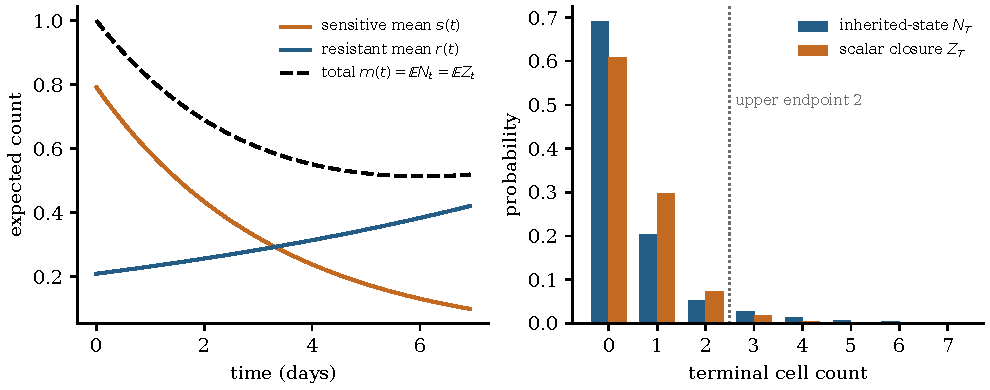
\includegraphics[width=\linewidth]{figures/distribution.pdf}
\caption{Numerical one-founder witness. Left: exact type-mean trajectories from~\eqref{eq:means}; the total mean coincides with the closure's mean for all $t$. Right: terminal count laws at $T$. The inherited-state process puts more mass both at extinction and at three or more cells while keeping the same mean.}
\label{fig:distribution}
\end{figure}

\begin{figure}[ht]
\centering
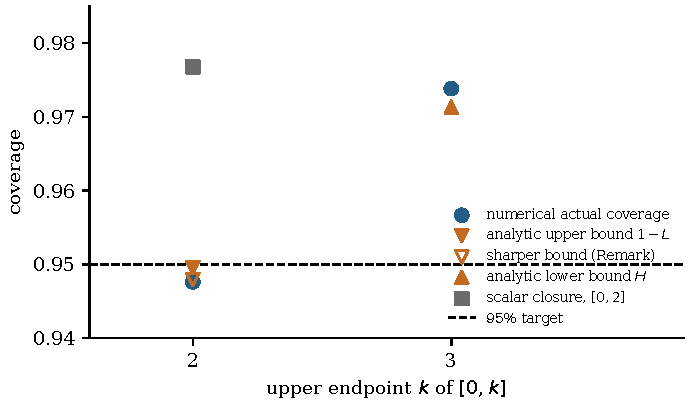
\includegraphics[width=.7\linewidth]{figures/coverage.pdf}
\caption{Actual coverage of $\{0,\dots,k\}$ at the two candidate endpoints. Dots: numerical values. Filled triangles: the certified upper bound $1-L$ at $k=2$ and lower bound $H$ at $k=3$; the open triangle is the sharper conventional bound of Remark~\ref{rem:geometric}. The square is the closure's own coverage of $\{0,1,2\}$.}
\label{fig:coverage}
\end{figure}

In an idealized assay with this preparation, accepting counts zero through two as the nominal $95\%$ prediction region misses more than $5\%$ of future outcomes, and raising the upper endpoint to three has a certified coverage above $97.13\%$. A real assay would additionally need plating, observation and parameter uncertainty accounted for before such a guarantee could be attached to it.

\subsection{Independent founders}
Table~\ref{tab:founders} and Figure~\ref{fig:founders} convolve the one-founder laws for $F$ up to $100$; the omitted actual mass at $F=100$ is below $10^{-13}$ with the $k=48$ coefficient system. The scalar central interval and its actual coverage are recomputed at every $F$. Coverage is not monotone in $F$, because integer endpoints move in jumps: it exceeds $95\%$ at $F=2$ and $F=3$, and rises slightly between $F=10$ and $F=20$. At $F=100$ the actual coverage is $0.8511$, consistent with the numerical limit $0.8488$ from the variances of Table~\ref{tab:witness}; both are below the certified bound $0.9308$ of Theorem~\ref{thm:clt}.

\begin{table}[ht]
\centering
\caption{Scalar central $95\%$ interval and its actual coverage for $F$ independent witness founders (numerical; the analytic bound constrains only the limit).}
\label{tab:founders}
\begin{tabular}{rcr@{\hspace{2.5em}}rcr}
\toprule
$F$ & Scalar interval & Actual coverage & $F$ & Scalar interval & Actual coverage\\
\midrule
1 & $[0,2]$ & $0.947598$ & 10 & $[1,10]$ & $0.903909$\\
2 & $[0,4]$ & $0.962995$ & 20 & $[4,18]$ & $0.904355$\\
3 & $[0,5]$ & $0.958707$ & 50 & $[16,37]$ & $0.868375$\\
5 & $[0,6]$ & $0.931584$ & 100 & $[38,67]$ & $0.851146$\\
\bottomrule
\end{tabular}
\end{table}

\begin{figure}[ht]
\centering
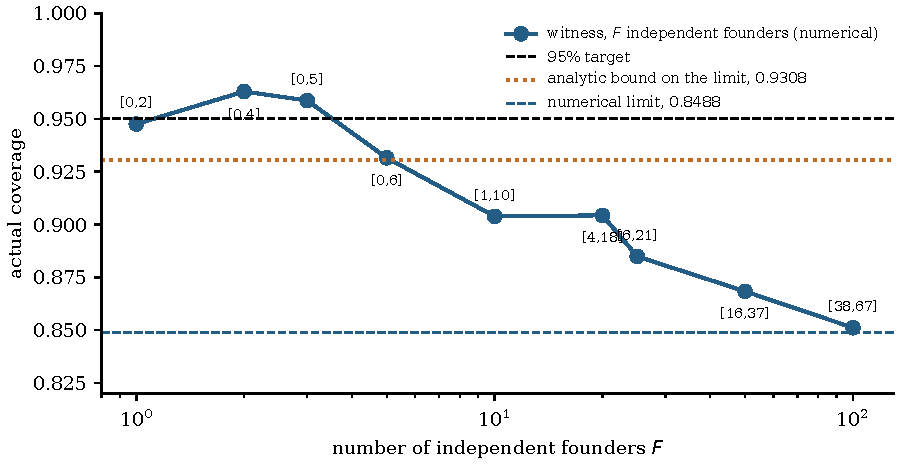
\includegraphics[width=.85\linewidth]{figures/founders.pdf}
\caption{Actual coverage of the scalar central $95\%$ interval against founder number (numerical, labels give the integer endpoints), the numerical limit $0.8488$, and the certified upper bound $0.9308$ on the limit. The bound constrains the limit, not every finite point.}
\label{fig:founders}
\end{figure}

\subsection{Scanning both switching rates}\label{sec:grid}
The witness's switching clocks are extreme. Figure~\ref{fig:grid} and Table~\ref{tab:grid} vary $\alpha$ over $10^{-4}$--$1$ and $\beta$ over $10^{-5}$--$1$ per day, holding $b=0.1$, $d=0.3$, $b_S=d_R=0$, $p=5/24$ and $T$ fixed, and recomputing the scalar central interval at every point. All lower endpoints are zero. Undercoverage of the scalar central interval occurs at seven of the thirty points: the six with $\alpha\le10^{-3}$ and $\beta\le10^{-3}$, and the point $(\alpha,\beta)=(0.01,0.01)$, where increasing $\beta$ from $0.001$ to $0.01$ moves the scalar upper endpoint from $3$ to $2$ and drops the actual coverage from $97.28\%$ to $94.79\%$. The variance ratio $v_Z/v_N$ (right panel, through the limit of Theorem~\ref{thm:clt}) varies smoothly and stays below $0.6$ over the whole slow-switching corner; the finite-count coverage does not follow it, because the integer quantile transitions dominate at one founder. A smooth variance surface therefore cannot serve as a surrogate for one-founder coverage, whereas it is exactly what governs the many-founder limit. The relevant asymptotic threshold is variance ratio one, not $55/64$; the latter is the certified witness value. The grid is synthetic and sparse; it is not interpolated into a certified boundary.

\begin{figure}[ht]
\centering
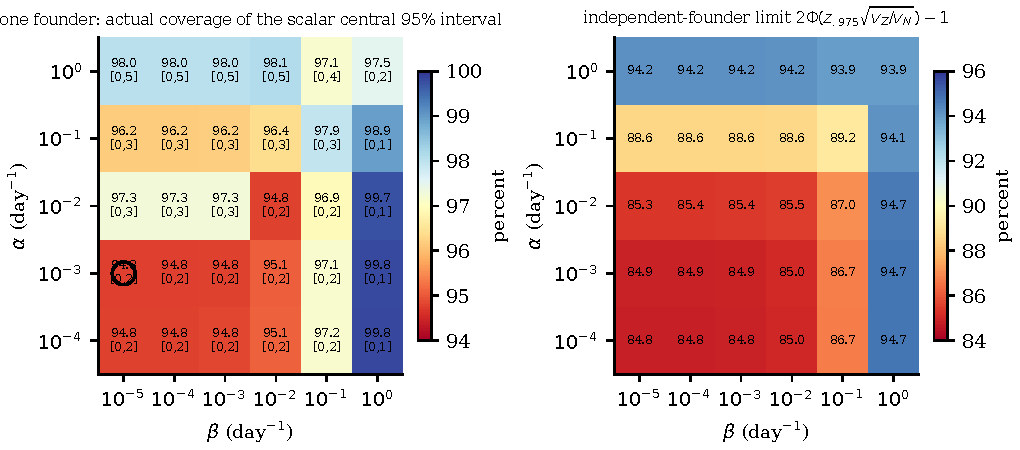
\includegraphics[width=\linewidth]{figures/grid.pdf}
\caption{Switching-rate scan at fixed $b=0.1$, $d=0.3$, $b_S=d_R=0$, $p=5/24$ and $T$ (numerical). Left: one-founder actual coverage of the scalar central $95\%$ interval, with the scalar interval printed in each cell; the circle marks the exact witness. Right: the independent-founder limit $2\Phi(z_{.975}\sqrt{v_Z/v_N})-1$ at the same points.}
\label{fig:grid}
\end{figure}

\begin{table}[ht]
\centering\small
\caption{One-founder actual coverage (percent) of the scalar central $95\%$ interval and, in brackets, its upper endpoint, on the switching grid of Figure~\ref{fig:grid}. Rows $\alpha$, columns $\beta$, in day$^{-1}$. Entries below $95\%$ are in bold.}
\label{tab:grid}
\begin{tabular}{r|rrrrrr}
\toprule
$\alpha\backslash\beta$ & $10^{-5}$ & $10^{-4}$ & $10^{-3}$ & $10^{-2}$ & $10^{-1}$ & $1$\\
\midrule
$10^{-4}$ & $\mathbf{94.79}$ [2] & $\mathbf{94.79}$ [2] & $\mathbf{94.82}$ [2] & $95.10$ [2] & $97.16$ [2] & $99.82$ [1]\\
$10^{-3}$ & $\mathbf{94.76}$ [2] & $\mathbf{94.76}$ [2] & $\mathbf{94.79}$ [2] & $95.07$ [2] & $97.14$ [2] & $99.81$ [1]\\
$10^{-2}$ & $97.26$ [3] & $97.26$ [3] & $97.28$ [3] & $\mathbf{94.79}$ [2] & $96.94$ [2] & $99.73$ [1]\\
$10^{-1}$ & $96.16$ [3] & $96.16$ [3] & $96.18$ [3] & $96.39$ [3] & $97.92$ [3] & $98.93$ [1]\\
$1$ & $98.02$ [5] & $98.02$ [5] & $98.03$ [5] & $98.11$ [5] & $97.14$ [4] & $97.51$ [2]\\
\bottomrule
\end{tabular}
\end{table}

\subsection{Positive rates in both states and day-scale switching}\label{sec:positive}
The exact witness converts negative net growth of sensitive cells into pure death and positive net growth of resistant cells into pure division. Table~\ref{tab:positive} relaxes this. The first two rows add sensitive division and resistant death at a common rate $e$ to the witness: at $e=0.001$ per day the undercoverage persists ($0.9481$); at $e=0.01$ it disappears for this interval criterion ($0.9520$). The remaining rows change the switching clocks and the zero rates together and follow the assay to $F=100$ founders. The middle row is the informative one: every event class has a positive rate, both isolated switching clocks have mean ten days, and the autonomous two-state relaxation time $1/(\alpha+\beta)$ is five days, yet the scalar central interval covers only $90.63\%$ at $100$ founders and its numerical limit is $90.07\%$. Its moments are $m(T)=0.55538$, $v_N=0.91188$, $v_Z=0.64471$ and $v_Z/v_N=0.70702$; the mean exceeds the witness box, so the witness's certified constants do not transfer, and this row is numerical evidence only. A separate forward calculation at cap $40$ agreed with the coefficient system within $3\times10^{-14}$, with retained overflow at most $1.2\times10^{-13}$. None of these rows is a fitted biological estimate.

\begin{table}[ht]
\centering\small
\caption{Perturbations of the witness with positive sensitive division and resistant death rates $b_S=d_R=e$ (numerical; $b_R=0.1$, $d_S=0.3$, $p=5/24$, horizon $T$ fixed). The limit column is $2\Phi(z_{.975}\sqrt{v_Z/v_N})-1$.}
\label{tab:positive}
\begin{tabular}{rrr@{\hspace{1.5em}}cr@{\hspace{1.5em}}crr}
\toprule
$\alpha$ & $\beta$ & $e$ & $F=1$ interval & coverage & $F=100$ interval & coverage & limit\\
\midrule
$0.001$ & $0.00001$ & $0$ & $[0,2]$ & $0.947598$ & $[38,67]$ & $0.851146$ & $0.848800$\\
$0.001$ & $0.00001$ & $0.001$ & $[0,2]$ & $0.948058$ & --- & --- & ---\\
$0.001$ & $0.00001$ & $0.01$ & $[0,2]$ & $0.951965$ & --- & --- & ---\\
$0.01$ & $0.01$ & $0$ & $[0,2]$ & $0.947846$ & $[38,68]$ & $0.868361$ & $0.854998$\\
$0.1$ & $0.1$ & $0.01$ & $[0,3]$ & $0.980862$ & $[41,72]$ & $0.906285$ & $0.900652$\\
$1$ & $0.01$ & $0.01$ & $[0,5]$ & $0.983256$ & $[119,171]$ & $0.948059$ & $0.943195$\\
\bottomrule
\end{tabular}
\end{table}

\begin{figure}[ht]
\centering
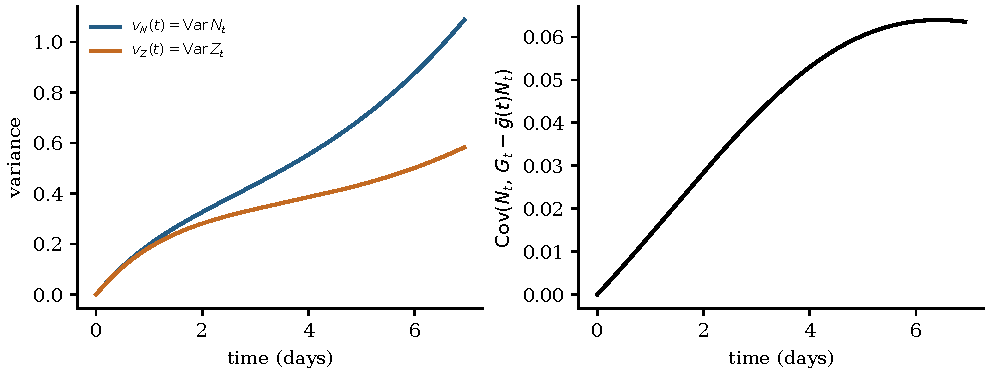
\includegraphics[width=\linewidth]{figures/defect.pdf}
\caption{The variance-defect identity for the witness (numerical). Left: $\Var N_t$ and $\Var Z_t$; both start at zero because the random founder type contributes $\Sigma(0)=p(1-p)C$ with $\ind^\top C\ind=0$. Right: the integrand $\Cov(N_t,G_t-\bar g(t)N_t)$ of~\eqref{eq:defect}, nonnegative throughout; the identity reproduces $v_N(T)-v_Z(T)=0.5043$.}
\label{fig:defect}
\end{figure}

\subsection{A source-linked control in which the closure covers}\label{sec:control}
To avoid presenting a counterexample to universal validity as evidence of universal failure, we retain a preparation in which the closure performs well. The pinned Figure~8 code of \citet{browningcode} specifies a two-type preparation with $\alpha=1$, $\beta=0.01$, $b_R=0.1$, $d_S=0.3$ per day, horizon $7$ days, initial count $\operatorname{Binomial}(1000,f)$ with $f=817\cdot614/(\pi\cdot4500^2)$, and initial resistant fraction the smaller root of $0.05\theta^2-0.57\theta+0.02=0$, about $0.0352$. This is a check of the two-type rate law and its scalar variant, not a reproduction of the full continuous-phenotype inference of \citet{browning2025}. The closure's central interval $[3,24]$ has actual coverage $0.95322$ (overflow $2.4\times10^{-8}$ at cap $60$); the mean is $11.32$ and the variance ratio is $1.034$. With fast switching, $\alpha T=7$, the founder state is forgotten within the horizon and the closure is adequate. The control has a different founder-count law and composition from the witness and is not a point on the founder curve of Figure~\ref{fig:founders}.

\section{Discussion}\label{sec:discussion}

\paragraph{Mechanism.} The closure fails because of correlated family growth from an inherited founder state. Conditional on a resistant founder, the family grows as a Yule process for the whole horizon with probability close to one; conditional on a sensitive founder, it almost surely dies or stays at one cell. The mixture has the same mean as the closure but more mass at zero and more mass at three or more. Proposition~\ref{prop:defect} makes this quantitative: the closure discards $\Cov(N,G-\bar gN)$, which is positive here throughout the horizon. The tail discrepancy is detected by seven explicit histories, the repair by a few more, and the founder-number limit by comparing two variances. None of these steps requires the joint law, which is why the whole argument is certifiable by hand and, in large part, by machine.

\paragraph{What the result does not show.} It does not show that mean-composition closures fail in general; Section~\ref{sec:control} and the fast-switching corner of Table~\ref{tab:grid} show them working. It does not show that inheritance always inflates the count variance relative to a closure; Corollary~\ref{cor:sign} gives a case with correlated families and no inflation. It does not identify a molecular mechanism, discriminate between forms of phenotypic memory, calibrate any cell line, or prescribe a treatment. The theorem is about prediction regions for a future count under known rates; parameter estimation, posterior prediction, plating randomness, measurement error, density dependence, non-exponential division times and shared environments are outside its assumptions and each can introduce its own calibration problem.

\paragraph{Implications for assay design.} Three measurements bear directly on whether a closure of this kind is adequate. Independent well or founder replicates estimate variability across genuinely independent units, whereas descendants within a well are not independent replicates. Founder-state information tests whether high-growth families originate preferentially in one initial state and whether that state persists through division. Perturbations of memory or turnover test whether the predicted count distribution, not just its mean, responds as the model says. Observed overdispersion can also come from variable plating efficiency, uncertain founder number, measurement error or between-well parameter variation, and a model comparison should not attribute all of it to inheritance. Where data permit, birth and death should be distinguished, because a net growth rate alone does not fix the turnover that drives count noise; the positive-rate rows of Table~\ref{tab:positive} were included for this reason.

\paragraph{Formal status.} The stochastic comparison is the principal result and is proved conventionally in full. Lean verifies the actual-process tail obstruction on a normalized, nonexplosive process law, the analytic bounds on the first-moment system, the explicit scalar law with its normalization and $332/343$ coverage, and the repaired threshold at the process level (Appendix~\ref{app:lean}). The identification of the unrestricted process means with the ODE solution and of the scalar jump process with Kendall's law are standard arguments that are proved in Section~\ref{sec:proof} and are not yet formalized. Completing them would strengthen the verification claim without changing the biological scope.

\appendix

\section{The polynomial certificate}\label{app:certificate}
Only one auxiliary inequality is needed for Lemma~\ref{lem:box}: $I=\int_0^1U(x)/D(x)^2\,\dd x\le9/4$ with $D(x)=5(1+x)^4+19$ and $U(x)=120(1+x)^6+1368(1+x)^2$. Let
\[
P(x)=\frac{25897}{10000}+\frac{3457}{2000}x-\frac{32099}{5000}x^2+\frac{179}{50}x^3 .
\]
Expansion gives the exact identity
\begin{equation}\label{eq:bernstein}
P(x)D(x)^2-U(x)=\sum_{j=0}^{11}a_j\,x^j(1-x)^{11-j}
\end{equation}
with the unnormalized Bernstein coefficients (no additional binomial factor)
\begin{align*}
(a_0,\dots,a_{11})=\Bigl(&\tfrac{2292}{625},\ \tfrac{41292}{625},\ \tfrac{10987}{625},\ \tfrac{39713}{625},\ \tfrac{12938273}{2500},\ \tfrac{28405139}{1250},\\
&\tfrac{54190307}{1250},\ \tfrac{26139962}{625},\ \tfrac{174528933}{10000},\ \tfrac{131199}{1250},\ \tfrac{58443}{2000},\ \tfrac{836124}{625}\Bigr).
\end{align*}
Every coefficient is positive and every basis term is nonnegative on $[0,1]$, while $D>0$, so $U/D^2\le P$ pointwise on $[0,1]$ and
\[
I\le\int_0^1P(x)\,\dd x=\frac{132541}{60000}=2.20901\ldots<\frac94 .
\]
The identity~\eqref{eq:bernstein} is an algebraic certificate, checked by exact expansion of both sides in \path{check_paper.py}, not a sampled inequality. The exact value of $I$ is $2.17876$.

\section{Lean verification status}\label{app:lean}
The conventional argument of Sections~\ref{sec:proof}--\ref{sec:founders} is self-contained. Its central components are additionally verified in Lean~4 (toolchain \lean{leanprover/lean4:v4.30.0}) against a frozen Mathlib manifest, with warnings treated as errors, in the namespace \lean{InheritedCellAssay} under \lean{proofs/InheritedCellAssay/}. The verifier exports the elaborated interface of each requested declaration and lists its axioms; the exported root declarations use only \lean{propext}, \lean{Classical.choice} and \lean{Quot.sound}, and no \lean{sorry}, admitted proposition or native numerical certificate enters. The formal clock is $\tau=(b+\beta)t$, so the horizon is $\log2$ and per-day rates are multiplied by $100000/10001$; the process carries an explicit unit-rate state-preserving event so that the total holding rate stays positive at extinction, which does not alter the observed population. Table~\ref{tab:lean} maps the mathematical components to their formal status at manuscript build.

\begin{longtable}{>{\raggedright\arraybackslash}p{0.42\linewidth}>{\raggedright\arraybackslash}p{0.52\linewidth}}
\caption{Claim-to-proof map. ``Compiled'' means strict verification with a receipt at manuscript build; ``conventional'' means proved in this paper only.}\label{tab:lean}\\
\toprule Mathematical component & Formal status\\
\midrule
\endfirsthead
\toprule Mathematical component & Formal status\\
\midrule
\endhead
Nonexplosive actual law; $\PP(N_T\ge3)>1/20$ (Section~\ref{sec:actualtail}) & Compiled: \lean{PositiveLaw.lean}, root \lean{PositiveTrajectory.actual_count_probability_gt}, stated for the normalized chronological measure of the two-type chain and the founder mixture; nonexplosion \lean{source_nonexplosion}; killed-history transport \lean{finite_le_actual} through \lean{FiniteClockProjection.clock_finite_projection}; exact seven-history value \lean{PositiveKilled.finite_failure_exact}. Receipt $61.7$~s, $85$ source files hash-matched.\\
Exact seven-history lower bound $L$ as a probability of the actual law & \LeanRepairExact\\
Repaired threshold $\PP(N_T\le3)\ge H$ at the process level (Section~\ref{sec:repair}) & \LeanRepair\\
Endpoint $2$ fails, endpoint $3$ succeeds, for the actual law (Corollary~\ref{cor:minimal}) & \LeanMinimal\\
First-moment ODE bounds~\eqref{eq:bounds1}--\eqref{eq:bounds2}; explicit nonnegative ODE solution; $m(T)\le11/20$; $A(T)\le2/5$ (Lemma~\ref{lem:box}) & Compiled: \lean{PositiveMoments.lean}, \lean{PositiveMomentConstruction.lean} (three-state killed chain construction of the solution), \lean{PositiveHorizon.lean} (\lean{endpoint_mean_upper}), \lean{PositiveBirthIntegral.lean} (\lean{birth_integral_bound}), reusing the Bernstein certificate of Appendix~\ref{app:certificate}.\\
Explicit scalar weights~\eqref{eq:weights}: nonnegativity, normalization, coverage $\ge332/343$ (Lemma~\ref{lem:scalar}, \eqref{eq:scalartail}) & Compiled: \lean{PositiveScalarLaw.lean} (\lean{weight_nonneg}, \lean{weight_pgf}, \lean{weight_normalized}, \lean{scalar_coverage_sharp}); a distribution-level result about the explicit weights built from the compiled mean and birth integral.\\
Backward rate identities~\eqref{eq:riccati} and rate bounds $0\le\lambda\le b$, $0\le\delta\le d$ & Compiled: \lean{PositiveScalarRates.lean} (\lean{backwardMean_derivative}, \lean{backwardBirth_derivative}, \lean{scalar_rate_bounds}).\\
Actual unrestricted means equal the ODE solution (Lemma~\ref{lem:moments}) & Conventional (Yule embedding, stopped Dynkin identity, dominated convergence); Lean bridge open.\\
Scalar jump process has the law~\eqref{eq:pgf} (Lemma~\ref{lem:scalar}) & Conventional (bounded backward test, stopped identity, bounded convergence); Lean bridge open.\\
Variance bounds, founder-number limit, variance-defect identity, low-count equations (Sections~\ref{sec:founders}--\ref{sec:thresholds}) & Conventional.\\
\bottomrule
\end{longtable}

Two cautions apply. Compilation of the explicit normalized scalar distribution does not by itself identify that distribution with the time-inhomogeneous jump process; that is the second open bridge. And the earlier no-switching comparison in the same repository (\lean{CountComparison.lean}, coverage $91/96$ and $187/192$) is a different theorem and is not used as a substitute for any positive-switching statement.

\section{Reproducibility}\label{app:repro}
The source package contains \path{main.tex}, \path{refs.bib}, the figures, and \path{check_paper.py}, which (i) replays in exact rational arithmetic every constant in Theorems~\ref{thm:main} and \ref{thm:clt}, Proposition~\ref{prop:variance}, Remark~\ref{rem:geometric}, Lemma~\ref{lem:box} and Appendix~\ref{app:certificate}, including the expansion of~\eqref{eq:bernstein} and the symbolic verification of the generator identities behind Proposition~\ref{prop:defect}; (ii) recomputes every numerical value of Section~\ref{sec:numerics} from the low-count system~\eqref{eq:coefficients} and the moment system~\eqref{eq:secondmoment}, cross-checks the witness and the positive-rate rows against the truncated joint forward equation, and evaluates the reference control from the pinned source; and (iii) draws Figures~\ref{fig:distribution}--\ref{fig:defect}. The whole run takes about two seconds. The Lean sources, receipts and the historical campaign ledger accompany the package separately.

\bibliographystyle{plainnat}
\bibliography{refs}

\end{document}
